\let\textcircled=\pgftextcircled
\chapter{Simulation Testing}
\label{chap:simulationtesting}

\initial{F}unctional and performance testing of the Kalman filter was done in MATLAB using the code described in appendix \ref{app:MATLAB}. This choice was made due to the intuitive graphical outputs produced as well as easy to use line breaks which allow careful tracking of the mathematics step by step. Simulations run for a fixed time length in discrete steps with data being stored for analysis afterwards.

\section{Data Generation}
Data generation comes in two stages, simulation of the drone's true movement and generation of sensory data.

\subsection{Movement Simulation}
The main lever for control of the drone's movement is through the control inputs. These can either be hard coded with constants, follow an equation over time, or be a constrained random variable. A mix of these were used over the course of general testing, however randomised inputs were considered best for final testing as they removed any question of bias. It could be argued that this is not representative of realistic drone behaviour however ability to work under worst case scenario is a good general starting point for testing of the filter. Control inputs were produced using a random number generator scaled to appropriate values. No official operational specifications exist for the drone used in this project, so maximum speed and acceleration were estimated based on the performance of similar drones in video \cite{hummingbird2015speed}. This shows a maximum speed around 14 m/s with an approximate acceleration of 3 m/s\textsuperscript{2}. Simulated movement will therefore be limited to 15 m/s with a maximum acceleration of 5 m/s\textsuperscript{2}. The process noise (the noise associated with drone adherence to control inputs) is more difficult to estimate and is dependent on factors such as weather conditions. Without real testing of the drone under specific conditions available to obtain noise readings, noise of equal proportion to the control inputs was used as a medium error estimate. \par

\subsection{Sensor Simulation}
Sensor data was provided by adding random noise to the true values thus producing noisy readings. Noise was scaled based on the sensors variance.\\

\smallskip
\noindent All random numbers were produced using MATLAB's \textit{randn} function that produces random numbers with a mean value of zero and variance of one.


\section{Results Analysis}
There are a number of metrics that can be used to measure the effectiveness of the filter. For this analysis we'll use the term \textit{average error}, this will be defined as the mean error in state estimate compared to the true value over every timestep of the simulation. These will generally be given separately for position, velocity and orientation. \par
	The code was run 500 times to produce the results detailed below and shown in figures \ref{fig:analysisposition} to \ref{fig:analysisorientation}. At 20 seconds per run with 0.1 second resolution the total time step sample size is 10,000 which was considered large enough to be representative. The raw values used to produce the aforementioned figures are available in appendix \ref{app:rawvalues}.\par
    A general trend over the data is that average extrapolated error and average filter produced error are very close. This is to be expected as the extrapolation step is generally good at short term estimation i.e. from one time step to the next. However if we took away the measurement data we would see that the filter would drift away from the true values due to accumulated error originating from the external noise. In this way drift is compensated for by the sensors, and even noisy data like that produced by the GPS can provide usable long term trends. This phenomenon is also used inside the inertial measurement units where the gyroscope is accurate but tends to drift over time, while the accelerometer is not so accurate but has no tendency to drift \cite{gade2009introduction}. \par
    Tables \ref{tab:rawvaluesnosensor} and \ref{tab:rawvaluesnosensordouble} in appendix \ref{app:rawvalues} show the effect that removing sensor data has on the filter estimates; larger average error that increases with simulation run time. Position estimate error can be seen to be especially increased, this is due to its derivation from velocity meaning that error is introduced two-fold through both the previous position and velocity estimate. 

\subsection{Average Positional Error}
The average measured error for position varies substantially between axes as evidenced in figure \ref{fig:analysisposition}. This can be attributed to the differences in sensory apparatus available for each. The y position has lowest average measured error due to using only relatively low variance ultrasonic and laser sensors. The x position has increased average measured error due to inclusion of the stereo camera disparity map in its available data. Addition of the very noisy GPS measurement to the z position sensory apparatus correspondingly raises the average measured error for that axis. As can be noted however, the difference in measured error does not adversely affect the filtered average error. Indeed the z position has a lower average error than the x position. This demonstrates that the Kalman filter is making efficient use of even very noisy data through appropriate weighting.

\begin{figure}[ht]
	\centering
	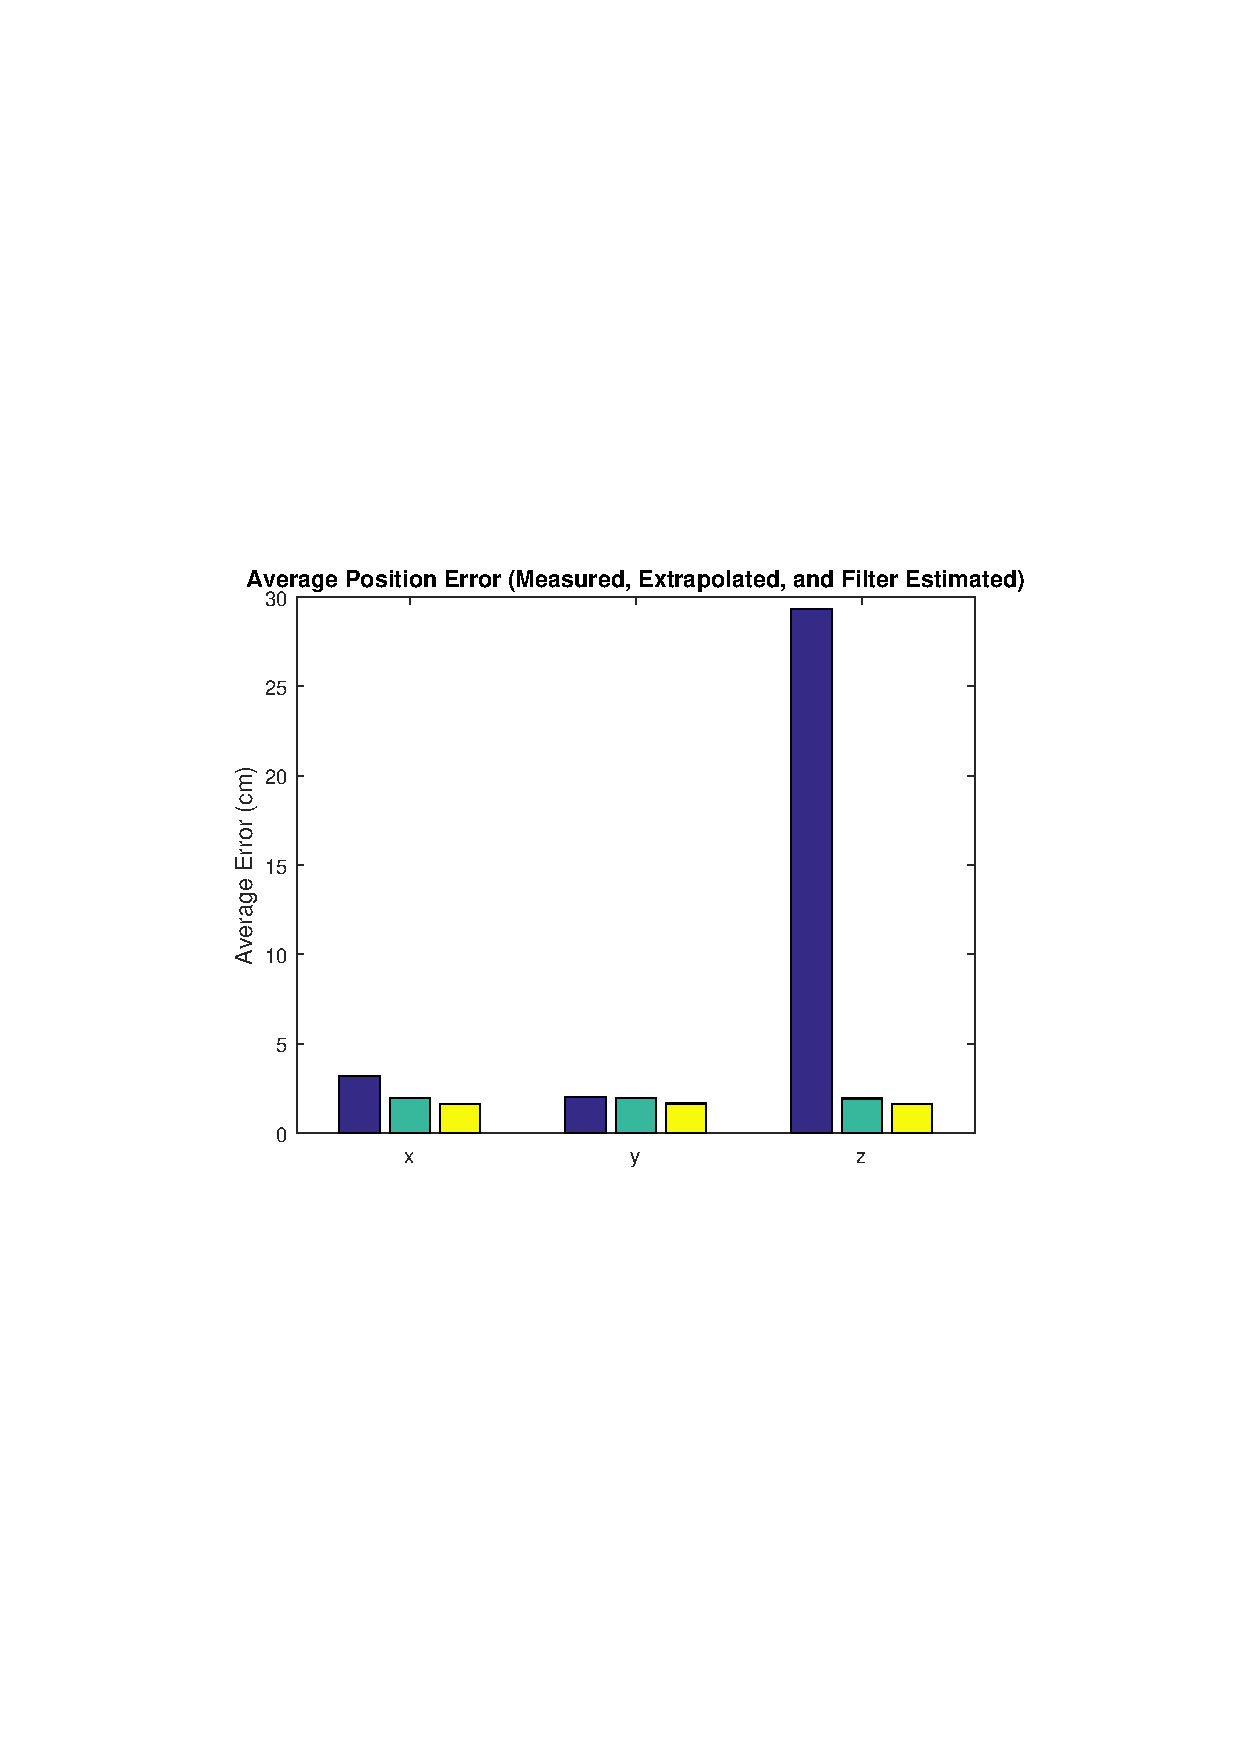
\includegraphics[height=0.40\textheight,trim={3cm 9.9cm 3cm 9.5cm},clip]{analysisposition.pdf}
	\mycaption[Position Results Analysis]{Bar chart showing average error from true results for measured, extrapolated and filter obtained position in the x, y and z axis.}
	\label{fig:analysisposition}
\end{figure}

\subsection{Average Velocity Error}
Average velocity error displayed in figure \ref{fig:analysisvelocity} shows a similar but even more exaggerated case of that seen in the z position data, very clearly showing that the extrapolation step contributes heavily to the much improved filter estimate. 

\begin{figure}[ht]
	\centering
	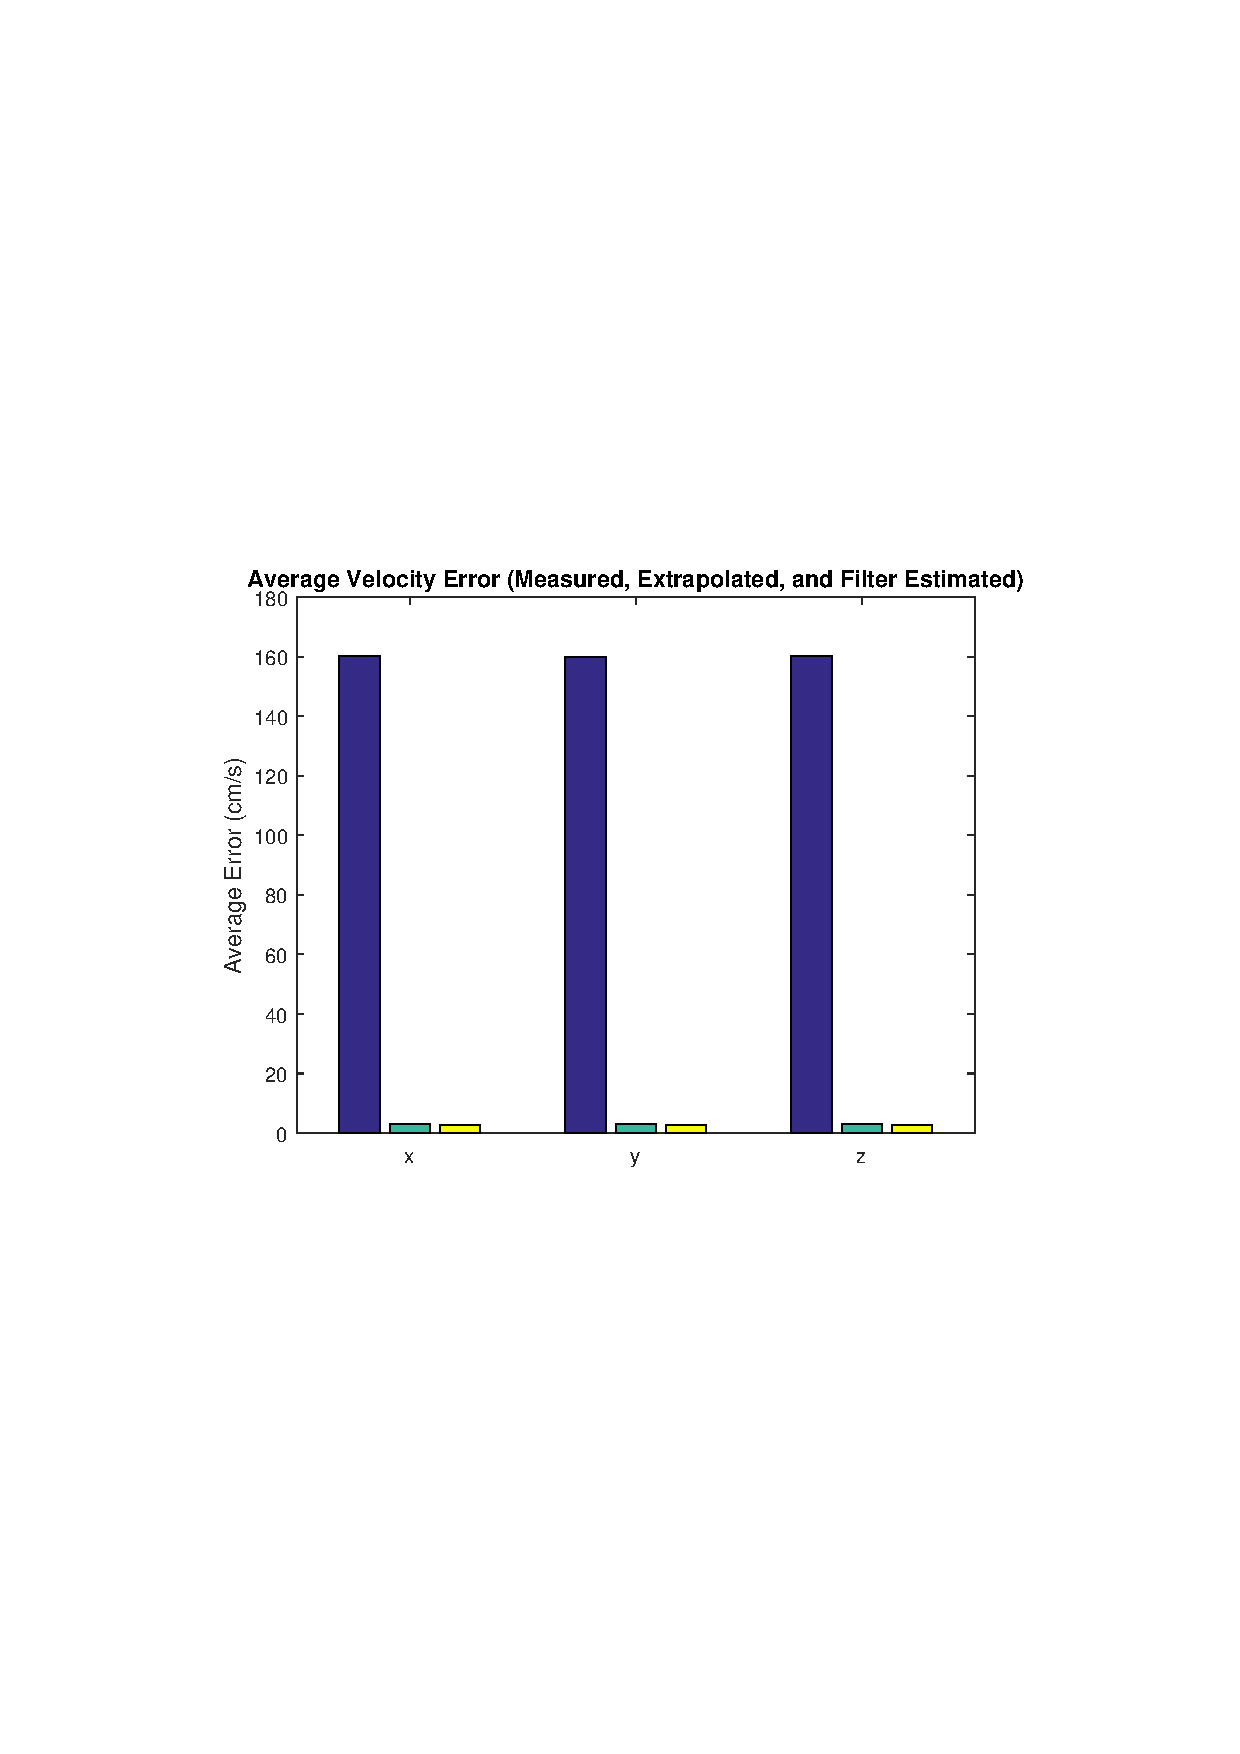
\includegraphics[height=0.40\textheight,trim={3cm 9.9cm 3cm 9.5cm},clip]{analysisvelocity.pdf}
	\mycaption[Velocity Results Analysis]{Bar chart showing average error from true results for measured, extrapolated and filter obtained velocity in the x, y and z axis.}
	\label{fig:analysisvelocity}
\end{figure}

\subsection{Average Orientation Error}
The orientation sensory apparatus does not incorporate any relatively high noise components, therefore it can be seen in figure \ref{fig:analysisorientation} that the extrapolation and filter estimates are not so distant from the measured as was the case in the previous examples. A marked improvement can however still be observed.

\begin{figure}[ht]
	\centering
	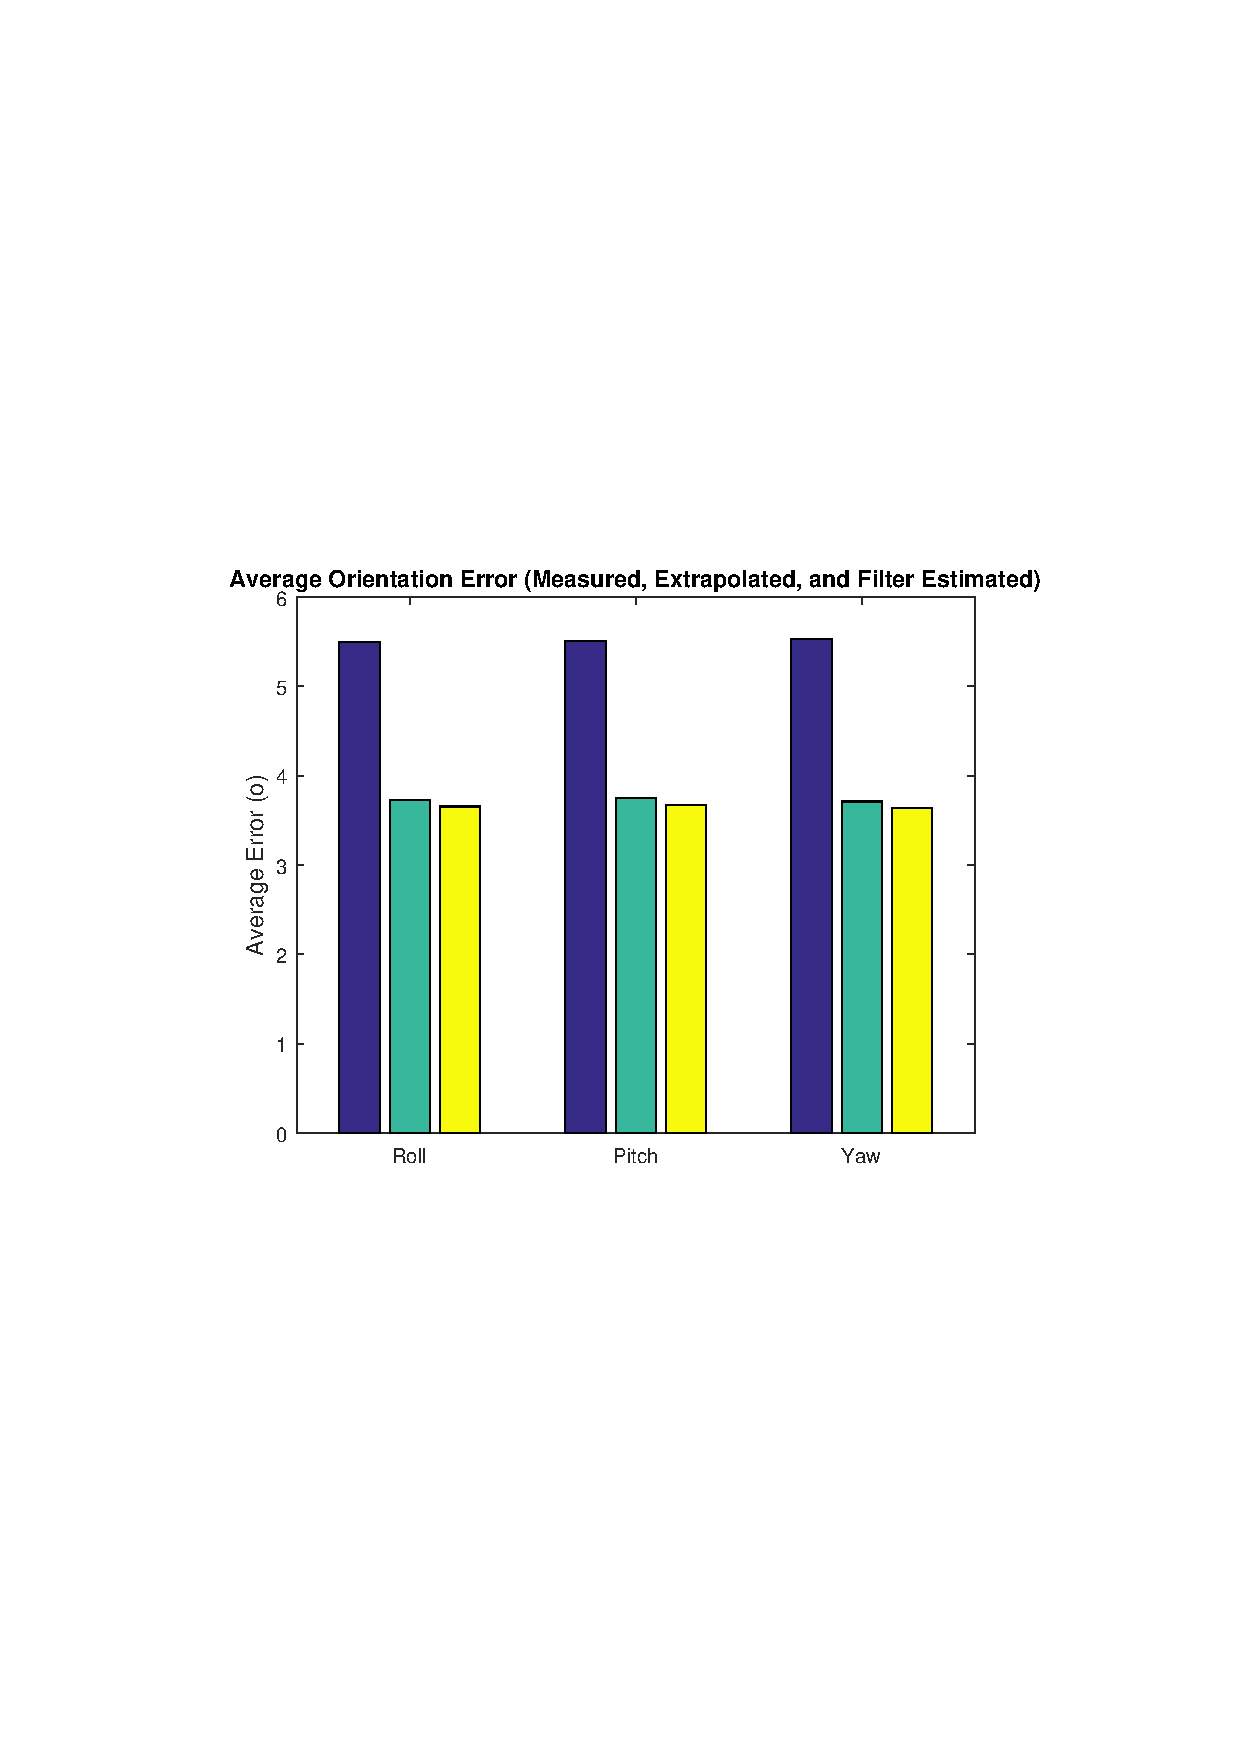
\includegraphics[height=0.40\textheight,trim={3cm 9.9cm 3cm 9.5cm},clip]{analysisorientation.pdf}
	\mycaption[Orientation Results Analysis]{Bar chart showing average error from true results for measured, extrapolated and filter obtained orientation in pitch, roll and yaw.}
	\label{fig:analysisorientation}
\end{figure}





























